
\chapter{Model-Based Clustering}
\label{chp:pmclust}

\section{Introduction}

Model-based clustering~\index{Model-Based Clustering}
is an unsupervised learning technique~\index{unsupervised learning}
and mainly based on finite mixture models to fit the data, cluster the data,
and infer the data~\citep{Fraley2002,Melnykov2010}. The major application of
model-based clustering focuses on Gaussian mixture models. For example,
$\bX_n$ is a random $p$-dimensional observation from
the Gaussian mixture model~\index{Gaussian mixture model}
with $K$ components which has a density
\begin{equation}
f(\bX_n; \bTheta) = \sum_{k = 1}^K \eta_k \phi_p(\bX_n; \bmu_k, \bSigma_k)
\label{eqn:gaussian_mixture}
\end{equation}
where $\phi_p(\cdot;\cdot,\cdot)$ is a $p$-dimensional Gaussian density,
$$
\bTheta = \{\eta_1, \eta_2, \ldots, \eta_{K-1},
\bmu_1, \bmu_2, \ldots, \bmu_K, \bSigma_1, \bSigma_2, \ldots, \bSigma_K\},
$$
is the parameter space,
$\eta_k$'s are mixing proportion, $\bmu_k$'s are centers of components, and
$\bSigma_k$'s are dispersion of components.

Suppose a data set $\bX = \{\bX_1, \bX_2, \ldots, \bX_N\}$ has
$N$ observations from
the Equation~(\ref{eqn:gaussian_mixture}), then the log likelihood is
\begin{equation}
\log L(\bTheta; \bX) = \sum_{n = 1}^N \log f(\bX_n; \bTheta)
\label{eqn:gaussian_mixture_logl}
\end{equation}
which is usually solved by the expectation-maximization (EM)
algorithm~\citep{Dempster1977}.~\index{EM algorithm}
After the EM algorithm is converged, let $\hat{\bTheta}$ is
maximum likelihood estimator of Equation~(\ref{eqn:gaussian_mixture_logl}),
then the maximum posterior probability
$$
\argmax_k
\frac{\hat{\eta}_k\phi_p(\bX_n; \hat{\bmu}_k, \hat{\bSigma}_k)
    }{f(\bX_n; \hat{\bTheta})}
$$
for all $n = 1, 2, \ldots, N$
indicates the membership of the data set $\bX$.


\pkg{mclust}~\citep{mclust}~\index{mclust} and
\pkg{EMCluster}~\citep{Chen2012EMClusterpackage}~\index{EMCluster}
are two main \proglang{R} packages implementing the EM algorithm for the
model-based clustering.
The \pkg{mclust} has several selections on models, and the \pkg{EMCluster}
implements the most complicated model (dispersions are all unstructured)
in a more efficient way, several initializations, and
semi-supervised learning.~\index{semi-supervised learning}
Both are assuming small $N$ and tiny $p$ and only run in serial with
sufficient memory.

Note that the k-means algorithm~\citep{Forgy1965}~\index{k-means}
equivalently assumes
$\eta_1 = \eta_2 = \cdots = \eta_K \equiv 1/K$ and
$\bSigma_1 = \bSigma_2 = \cdots = \bSigma_K \equiv \bI$
in the Equation~(\ref{eqn:gaussian_mixture}) where
$\bI$ is an identity matrix.
The k-means algorithm is a restricted Gaussian mixture model such that
it can be implemented in a simplified way of the EM algorithm.
However, the cluster results are always unrealistic, unable to infer,
and sometimes seriously with high classification errors.


\subsection{Parallel Model-Based Clustering}

\pkg{pmclust}~\citep{Chen2012pmclustpackage}~\index{pmclust}
is an \proglang{R}
package for parallel model-based clustering based on mixture Gaussian models
with unstructured dispersions.
The package assumes data are distributed on several machines, therefore,
some gathering and reducing are necessary at some stages of EM algorithm.
An expectation-gathering-maximization (EGM)
algorithm~\citep{Chen2013}~\index{EGM}
is established for minimizing communication and data moving between machines.
There are four variants of EGM-like algorithms implemented in \pkg{pmclust}
include EM, AECM~\citep{Meng1997}~\index{AECM},
APECM~\citep{Chen2011}~\index{APECM},
and APECMa~\citep{Chen2013}~\index{APECMa}. The variants are trying to yield
better convergent rate and less computing time than the original EM algorithm.
A simple k-means algorithm is also implemented in \pkg{pmclust}.

The \pkg{pmclust} is the first
\proglang{pbdR} application, and the first
\proglang{R} package in SPMD to analyze distributed data in Terabytes level.
Originally, it is designed for analyzing Climate simulation outputs (CAM5)
as discussed in Section~\ref{sec:pbdNCDF4_introduction}, and
is a product for the project
``Visual Data Exploration and Analysis of Ultra-large Climate Data''
supported by U.S. DOE Office of Science.

The \pkg{pmclust} initially depended on \pkg{Rmpi}, but
designed in SPMD approach rather than in master/workers approach even before
\proglang{pbdR}.
Later, it migrates to use \pkg{pbdMPI}~\citep{Chen2012pbdMPIpackage}
for performance issues of larger machines.
So, by default, the package assumes data are stored in
SPMD row-major matrix format.
Currently, the package also fully utilizes
\pkg{pbdSLAP}~\citep{Chen2012pbdSLAPpackage},
\pkg{pbdBASE}~\citep{Schmidt2012pbdBASEpackage}, and
\pkg{pbdDMAT}~\citep{Schmidt2012pbdDMATpackage}
to implement algorithms in \code{ddmatrix} format.
Table~\ref{tab:pmclust_algorithm} lists the current implementations.
\begin{table}[h]
\centering
\caption[Parallel Mode-Based Clustering Algorithms in \pkg{pmclust}]{
Parallel Mode-Based Clustering Algorithms in \pkg{pmclust}}
\label{tab:pmclust_algorithm}
\begin{tabular}{ccc} \hline\hline
Algorithm & SPMD & \code{ddmatrix} \\ \hline
EM        & yes  & no              \\
AECM      & yes  & no              \\
APECM     & yes  & no              \\
APECMa    & yes  & no              \\
k-means   & yes  & yes             \\ \hline\hline
\multicolumn{3}{c}{
Based on \pkg{pmclust} version 0.1-4}
\end{tabular}
\end{table}


\section{The {\it Iris} Dataset}

The \code{iris}~\citep{Fisher1936}~\index{iris} dataset in \proglang{R}
is a tiny dataset for 50 iris flowers from each of three species of iris
which are {\it Iris setosa}, {\it Iris versicolor}, and {\it Iris virginica}.
The dataset has in total 150 rows and five columns including
four features (sepal length and width, petal length and width) and
class of species.
We take the first four columns of \code{iris} to form $\bX$ matrix
where each row can be
classified in three groups by the true id (the fifth column of \code{iris})
for supervised learning,
or clustered in three groups by algorithms for unsupervised learning.
Note that the dimension of $\bX$ is $N = 150$ by $p = 4$.

Figure~\ref{iris_pairs} shows the pair-wised scatter plot for all features
denoted on the diagonal, and classes are indicated by colors. Each panel
plots two features on x and y axes. It is clear
that \code{Petal.Length} can split three species in two groups. However,
one of the group is mixed with two species and can not be distinguished by
any of these four features.
\begin{figure}[h!bt]
  \centering
  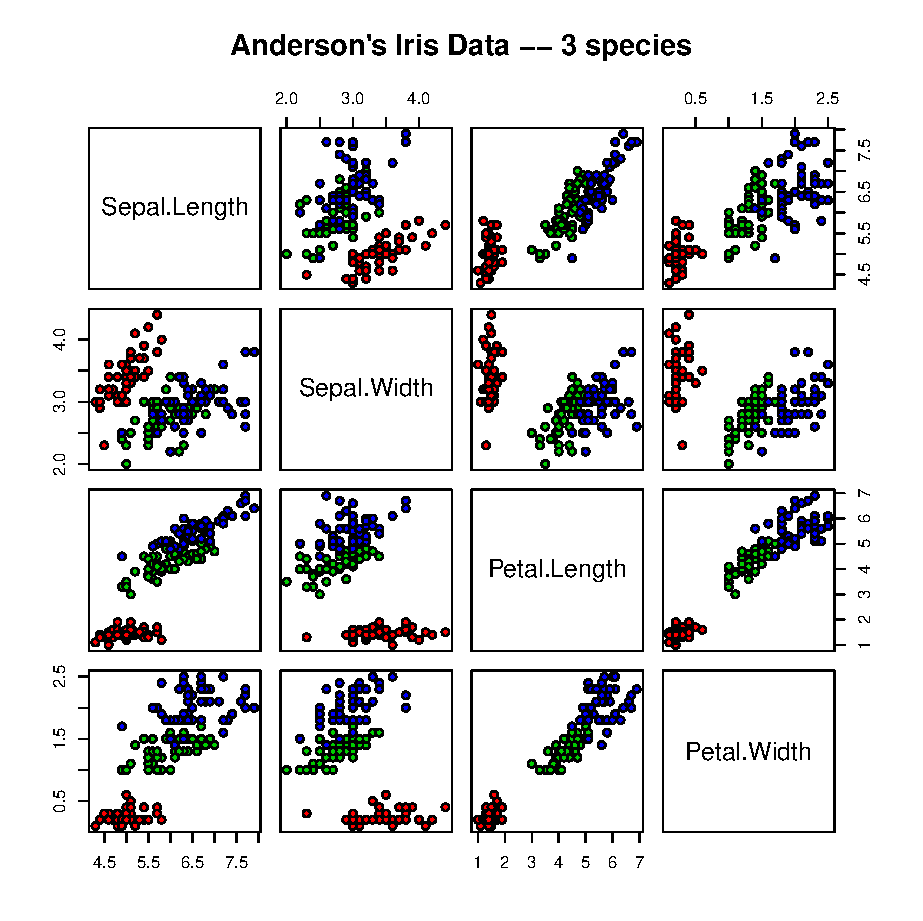
\includegraphics[width=6.5in]{pbdDEMO-include/pics/iris_pairs.pdf}
  \vspace{-1.5cm}
  \caption[Iris pair-wised scatter plot]{
    Iris pair-wised scatter plot. {\it Iris setosa} is in red,
    {\it Iris versicolor} is in green, and {\it Iris virginica} is in blue.
  }
  \label{fig:iris_pairs}
\end{figure}


From the supervised learning point view, the empirical estimation for
$\bTheta$ from data will be the best description for the data assuming
the true model is Gaussian mixture. The demo code \code{iris_overlap} in
\pkg{pbdDEMO} quickly suggests the overlap level of three
iris species. It can be obtained by
\begin{Code}[title=R Code]
R> demo(iris_overlap, 'pbdDEMO', ask = F, echo = F)
\end{Code}
which utilize \code{overlap} function of \pkg{MixSim}~\citep{Melnykov2012}.
The output is
\begin{CodeOutput}
R> (ret <- overlap(ETA, MU, S))
$OmegaMap
             [,1]         [,2]       [,3]
[1,] 1.000000e+00 7.201413e-08 0.00000000
[2,] 1.158418e-07 1.000000e+00 0.02302315
[3,] 0.000000e+00 2.629446e-02 1.00000000

$BarOmega
[1] 0.01643926

$MaxOmega
[1] 0.0493176

$rcMax
[1] 2 3

R> (levels(iris[, 5]))
[1] "setosa"     "versicolor" "virginica"
\end{CodeOutput}
The \code{OmegaMap} is a map of pair-wised overlap of three species
where 1, 2, 3 are {\it Iris setosa}, {\it Iris versicolor}, and
{\it Iris virginica}, respectively.
The outputs also indicate that the averaged pair-wised overlap (\code{BarOmega})
is about $1.6\%$, and the maximum pair-wised overlap (\code{MaxOmega}) is
about $4.9\%$ among these three iris species. Also,
the maximum occurs at 2 ({\it Iris versicolor}) and 3 ({\it Iris virginica})
indicating these two species are partly inseparable given these four features.

For unsupervised learning point view, such as model-based clustering,
suppose we were blinded to the true class ids or assuming
the fifth column of $\bX$ is unobserved,
but only use the four
features to form the model and cluster the data.
Note that
{\it Iris versicolor} and {\it Iris virginica} are partly inseparable,
so misclassification can happen at the overlap region.
We validate the results by comparing the clustering ids
to the true class ids using adjusted Rand index~\citep{Hubert1985}.
The adjusted Rand index has values between 1 and -1 where 1 means perfect
match otherwise less than 1. The function \code{RRand} in \pkg{MixSim}
also provide the adjusted Rand index.

In order to show the unsupervised learning, we then use the \code{iris}
in the following steps to show the scalability of \pkg{pmclust}.
We first illustrate the \code{iris} in a serial code:
\begin{itemize}
\item decompose the $\bX$ on principal components,
\item project the $\bX$ on the first two dimension with largest variation,
\item visualize the $\bX$ on the x-y plane,
\item label $\bX$ with true ids, and
\item label $\bX$ with estimated ids clustered by algorithms.
\end{itemize}
Then, we repeat these steps in SPMD code and in \code{ddmatrix} code
to show the similarity of codes.
This shows that \pkg{pmclust}
can cluster data from very tiny dataset on single machines, but there is
no difficulty to scale to very large dataset on supercomputers.




\subsection{{\it Iris} in Serial Code}




\subsection{{\it Iris} in SPMD Code}




\subsection{{\it Iris} in \code{ddmatrix} Code}




\section{Exercises}
\label{sec:pmclust_exercise}

\begin{enumerate}[label=\thechapter-\arabic*]
\item

\end{enumerate}

